\frame{
\frametitle{Algoritmo Genético}
\begin{block}{}

%\begin{lstlisting}
\begin{algorithm}[H]
\SetKwBlock{Procedimento}{Procedimento}{fim}

%Algorithm: GA(n, \ki, \mu)
\Procedimento{
  %// Initialise generation 0:
  $k \leftarrow 0$, $P_k \leftarrow n$ indivíduos aleatórios\;
  %// EvaluatePk:
  %\Para{cada $i$ em $P_k$}
  %Compute fitness(i) for each i ∈ Pk;
  %Computar a $avaliacao(i)$ para cada $i$ em $P_k$\;
  %while fitness of fittest individual in Pk is not high enough;
  %\Enqto{a $avaliacao(i)$ de cada $i$ em $P_k$ não for boa o suficiente}{
  \Enqto{$avaliacao(i) < desejado$ de cada $i$ em $P_k$}{
    %// Create generation k + 1:
    %// 1. Copy:
    %Select (1−χ)×n members ofPk and insert into Pk+1;
    Selecionar os $(1 - \chi) \times n$ membros com maior $avaliacao(i)$ de $P_k$ e inserir em $P_{k+1}$\;
    %// 2. Crossover:
    %Select χ×n members of Pk; pair them up; produce offspring; insert the offspring into Pk+1;
    Selecionar $\chi \times n$ membros de $P_k$, pareá-los e inserir a cria em $P_{k+1}$\;
    %// 3. Mutate:
    %Select µ×n members of Pk+1; invert a randomly-selected bit in each;
    Selecionar os $\mu \times n$ membros de $P_{k+1}$ com maior $avaliacao(i)$ e inverter um bit aleatório de cada membro\;
    %// Evaluate Pk+1:
    %Compute fitness(i) for each i ∈ Pk;
    %Computar a $avaliacao(i)$ para cada $i$ em $P_{k+1}$\;
    %// Increment:
    %k := k + 1;
    $k \leftarrow k + 1$\;
  }
%return the fittest individual from Pk;ut your code here.
  \Retorna{membro $i$ em $P_k$ com maior $avaliacao(i)$}
}
\caption{Pseudo código de um Algoritmo Genético}
\end{algorithm}
\end{block}
}

\frame{
\frametitle{Algoritmo Genético}
\begin{block}{}
\begin{figure}[H]
\centering
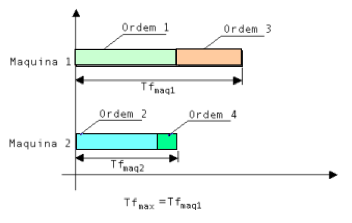
\includegraphics[width=6cm]{figuras/ga_exemplo}
\caption{Exemplo de problema resolvido com Algoritmo Genético.}
\end{figure}
\end{block}
}
